\documentclass[conference]{IEEEtran}
\IEEEoverridecommandlockouts
% The preceding line is only needed to identify funding in the first footnote. If that is unneeded, please comment it out.
\usepackage{cite}
\usepackage{amsmath,amssymb,amsfonts}
\usepackage{algorithmic}
\usepackage{graphicx}
\usepackage{textcomp}
\usepackage{xcolor}
\usepackage{array}
\def\BibTeX{{\rm B\kern-.05em{\sc i\kern-.025em b}\kern-.08em
    T\kern-.1667em\lower.7ex\hbox{E}\kern-.125emX}}
\usepackage[caption=false,font=footnotesize]{subfig}

\begin{document}
\graphicspath{{images/}}
% and their extensions so you won't have to specify these with
% every instance of \includegraphics
% \DeclareGraphicsExtensions{.pdf,.jpeg,.png}

\title{Application of Transformers for Oil Well Production Forecasting}

\author{\IEEEauthorblockN{1\textsuperscript{st} Pedro Henrique Cardoso Paulo}
\IEEEauthorblockA{\textit{Mechanical Engineering Department} \\
\textit{Petrobras and PUC-Rio}\\
Rio de Janeiro, Brazil \\
pedrorjpaulo.phcp@gmail.com}
\and
\IEEEauthorblockN{2\textsuperscript{nd} Felipe da Costa Pereira}
\IEEEauthorblockA{\textit{Mechanical Engineering Department} \\
\textit{Petrobras and PUC-Rio}\\
Rio de Janeiro, Brazil \\
felipecostapereira@gmail.com}
\and
\IEEEauthorblockN{3\textsuperscript{rd} Helon Vicente Hultmann Ayala}
\IEEEauthorblockA{\textit{Mechanical Engineering Department} \\
\textit{PUC-Rio}\\
Rio de Janeiro, Brazil \\
helon@puc-rio.br}
}

\maketitle

\begin{abstract}
In the oil and gas industry, long-term development strategies as well as short-term operational decisions rely on well monitoring data. In recent years, 
this industry has benefited from machine learning techniques as the availability and quality of oil field data, allowing the application of data-driven models 
to fit and predict field behaviour and provide better business decisions. Among the variables of interest, the production rates are worth studying due to its 
connection to the revenue and uncertainties associated to its determination.

This study makes use do the transformer neural network architecture in order to perform the production forecast of an oil well from the Volve dataset. 
The results are compared with other possible solutions for the task, such as the system identification approach using different regressors. An statistical analysis
of the model and hyperparameter investigation is also presented. 

The final models showed interesting results when compared to the real data, with the transformer being the best model in the base case.
The statistical tests performed indicated low impact of the memory size and more tendency of outlier models in case of a large number of encoder layers
for a dataset comprised of one single well with relatively few samples. The transfer learning test showed promising results in OSE predictions, but failed
in a Free-run simulation, which is the main interest of the work, with further tests to improve being needed.

%This study provides a black box system identification approach to overcome these limitations and address the well monitoring challenges, being an alternative to conventional well flow rates estimation and pressure-temperature gauges unavailability. We focused in well flow rates estimation based on operational available input data and aiming missing production history, reservoir management and production forecast applications: a digital twin for an oil well.

%A python implemented class was deployed in order to allow the use of any standard regressor to predict time series values, once a set of input/output lags is selected. This flexibility improves the implementation of those models and makes the comparison between model types more feasible. The MLP regressor, as well as other types of regressors showed a good accuracy in predicting rates for a real field well application, where the dynamics are difficult to predict due to the wide range of operational conditions.
\end{abstract}

\begin{IEEEkeywords}
transformers, pytorch, neural network, oil and gas, production forecast, digital twin.
\end{IEEEkeywords}

\section{Introduction}\label{sec:section_introduction}
% no \IEEEPARstart

% INTRODUCAO
%\color{black}
Well monitoring and production rates estimations compose the reservoir management activity 
and have a major role in the oil and gas industry. Being able to accurately forecast the 
production of a well or an oilfield is a constant need on the oil and gas industry in order 
to assess the economic value of its assets, calculate royalties to be paid and perform an 
effective reservoir management strategy that will increase the value extracted from the oil 
field \cite{alakeely2022simulating}.

In most offshore production facilities, the separation of the three phases (oil, gas and water)
of the wells is performed only for the total production of the unit, as the space available 
for the separation vessels is limited. A second separation system is usually available to 
separate fluids of a single well in order to have an accurate measurement of its three phases 
flow rates. This vessel is called test separator and this operation of measuring flow rates is 
known as well test. As the separator test measures are obtained for a single well at a time, 
most part of the time the well flow rates are not being continuously acquired. The full 
historic production flow rates for each of the connected wells, is then, uncertain as it 
is usualy reported as an apportionment of the total production. An alternative to the 
traditional well test based apportionment is the use of multi phase flow meters, however, 
since multi phase flow is complex, turbulent, and chaotic, the acquisition of accurate, 
reliable, and repeatable rate measurements can be a challenge \cite{Okotie2016}.

Due to the challenges associated to the determination and forecasting of production rates per 
well, production predictions are normally performed by using simulation models based on first 
principles. These models are built and maintained by qualified engineers by using pressure and 
temperature data taken from sensors positioned in key points of the well, some of which are 
displayed schematically in figure \ref{fig:pressureSensors}. Adjusting the reservoir model in 
order to correctly match the actual dynamic historic behaviour is the process known as history 
match \cite{alakeely2022simulating}. Li et al. \cite{Li2019} comment that this approach, due 
to some simplified assumptions, may generate uncertain models and also cites the pressure 
dependency of the flow rate as input, an already uncertain variable, as a major limitation. 
The dependency of well sensors for the history match can also be a 
challenge, since there is always a risk of losing some measurements. As an example, the 
donwhole pressure is one of the most important variable to provide useful information for 
management and oil recovery of the oil field \cite{camponogara2010automation} but the PDG 
sensor responsible for its measurement has a high failure rate. Those systems for measuring 
pressure and temperature historically exhibited a low reliability \cite{Gisbergen2001} and, 
in offshore wells, the replacement of such equipment once it's damaged is not a common 
operation due to the high costs associated with the workover operation and high environmental 
risks \cite{Freitas2021}. In that case, reservoir management becomes more challenging and lack 
of information may hinder decisions that depend on long-term predictions. 

\begin{figure}[htbp]
\centerline{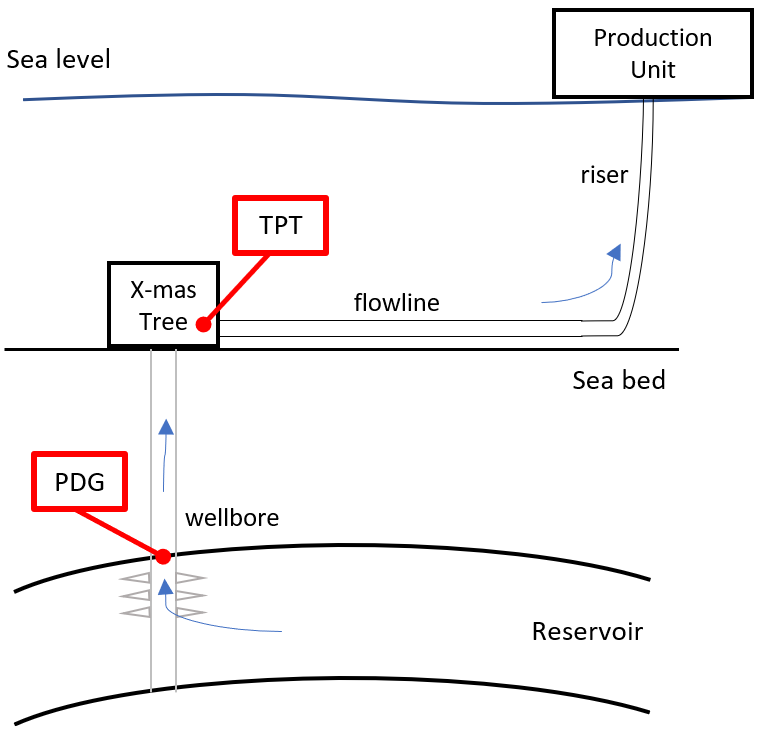
\includegraphics[width=3.0in]{wellScheme.png}}
\caption{Typical offshore well and its pressure-temperature sensors: PDG (located downhole) and TPT (located in the X-mas tree, the sea bed equipment which connects the well with the flowline).}
\label{fig:pressureSensors}
\end{figure}

% LITERATURE REVIEW
Reservoir management area has recently benefited from machine learning methods that emerged as 
powerful tools to address these key challenges \cite{alakeely2022simulating}, posing as an 
alternative to the conventional first principles approach. Many studies have addressed the 
problem of predicting well rates and reservoir monitoring by the use of artificial intelligence 
techniques such as machine learning methods. According to Alakeely et al. \cite{AlakeelyGA2022}, 
these models are powerful tools for tasks where the actual model between the input and output variables 
is not well defined or does not exist, and where forward modeling is well defined, but the inverse model 
is challenging. The difficulty in modeling the dynamic behaviour of those systems is that they present 
a wide range of operating conditions what makes the prediction task a challenging one \cite{Freitas2021} 
\cite{Apio2019}. This happens because the physical phenomena that happen in a certain time window on a 
well production history are not expected to be repeated over time as the water and gas fractions tend to
rise and the pressure levels tend to monotonically decrease. These variables are responsible for changing 
the well behavior in several parameters, like productivity index, phase viscosities and densities. 

Alakeely and Horne \cite{Alakeely2021} proposed a Deep Learning method using surface measurements 
to predict well flow rates. Also in \cite{Alakeely2021}, autoencoders were used to generate 
additional inputs and the results were compared to classic Gilbert correlation methods. 
Cao et al. \cite{CaoQ2016} used a single-layer fully-connected neural network to predict the 
production rates of existing wells, but also tried o add information from the geologic contex 
in order to predict new wells.

As already mentioned, well pressure and temperature sensors, in case of fail, are unlikely to 
be replaced in a short period thanks to economical and environmental reasons. In that sense, 
soft sensors models emerge as an alternative to replace a sensors such as the PDG 
\cite{Aguirre2017}. A study on PDG soft sensors is provided by Aguirre et al. in 
\cite{Aguirre2017} using NARMAX, neural networks, committee machines, unscented Kalman filters 
and filter banks models. Aguirre et al. \cite{Aguirre2017} also show the key-problems in 
developing soft-sensors and reveal the strengths and weaknesses of each alternative, based on 
diverse oil wells considered. An application of Echo State Network to model well downhole and 
riser inlet pressure by using surface and subsea valves position as input variables is 
provided by Jourdanou et al. \cite{JORDANOU2019} where the data is generated by a flow 
simulator and the framework is then used for nonlinear model predictive control (NMPC) 
purposes. Li et al. \cite{Li2019} also modeled the downhole pressure with deep learning 
models, searching for the best architecture to represent short-term transients and long-term 
variations.

Still on the matter of time series regression and foreacasting, the transformer neural network architecture
is seen as a competitive and flexible architecture to perform the task. It was originally proposed 
for the task of NLP, which can be considered a complex time series problem, and has considerable advantages
when compared to methods such as NARMAX and other deep learning techiniques such as RNN ans LSTM regarding
the time window it can consider and paralelization of the training. Pazouki and Farsani \cite{transformers_ts_forecasting}
used an adapted version of the architecture in multiple benckmark datasets and obtained better or equivalent results when compared to
other methods. Zerveas et al. \cite{multivariate_ts_forecasting} propose not only the use of the transformer architecture
for time series tasks, such as regression and classification, but also a generalistic framework for working with multivariate
time series using the architecture, claiming that it would be possible to also perform an unsupervised pre-training of the network
by using it in autoregression tasks. Zerveas et al. \cite{multivariate_ts_forecasting} also apply their proposed architecture to various
time series problems, obtaining better or close results when compared to other methodologies.

% Critial analysis, paper goals, and original contributions
The main goal of this work is to investigate the applicability of the transformer architecture
to the task of creating a black-box model for production forecasting using real data from Volve
dataset \cite{volve_data}. This approach will be compared with other forecasting models created
using the system identification methodology. The statistical variation of the final model, and 
the impact of some hyperparameters of the proposed simplified transformer architecture will also 
be investigated.


%The main contribution of this paper is the application in a real field well case with challenging dynamics to be identified and the methods capability to be easily generalized to any standard scikit learning regressor class.

% paper organization
This paper is organized as follows: in section \ref{sec:section_case_study} we describe the case 
study, the dataset characteristics and the variables used. In section \ref{sec:compared_approaches}, 
both the system identification approach and the transformer architecture are briefly explained and compared.
In section \ref{sec:section_method}, training and comparison methodology is 
detailed and in \ref{sec:section_results} a discussion is conducted regarding the most important 
results achieved. Finally, a conclusion is made in section \ref{sec:section_conclusion} as well as 
future works and analysis recommendation.


\section{Case study}\label{sec:section_case_study}

The Volve field is an oilfield on the North Sea discovered in 1993. The field was operated by 
Equinor who started production in 2008 from a Middle Jurassic age sandstone reservoir 
\cite{volve_info}. The field was shut down on 2016, with its production facilities being 
removed in 2018.

An open-source dataset containing exploration and production data from this field, the Volve 
dataset, was then disclosed by operator Equinor, in 2018. The dataset contains geological, 
geophysical, seismic and logging data, reservoir models and reports from the Volve field 
\cite{volve_data}. The dataset also includes production data from the reservoir, 6 production 
wells and 1 injection well, which includes dynamic data of pressure and temperature sensors, 
choke sizes and production flow rates. Some of the variables available on the dataset for each 
production well and its definitions are listed on the table \ref{tab:volve_variables}.

\begin{table}[htbp]
\caption{Volve Dataset variables and definitions used on this case}
\begin{center}
\centering
\begin{tabular}{|c|c|}
\hline
\textbf{Variable}&{\textbf{Definition}} \\
\hline
BORE\_OIL\_VOL             & Average oil flow rate on \\
                           &  one day of production\\
\hline
BORE\_WAT\_VOL             & Average water flow rate on \\
                           & one day of production\\
\hline
BORE\_GAS\_VOL             & Average gas flow rate on \\
                           & one day of production\\
\hline
BORE\_LIQ\_VOL            & Average liquid flow rate on \\
                           & one day of production\\
\hline
AVG\_DOWNHOLE               &  Daily average of the downhole\\             
\_PRESSURE                  &  pressure measured by the permanent\\
                            &  downhole gauge (PDG)\\
\hline
AVG\_DOWNHOLE               &   Daily average of the downhole\\
\_TEMPERATURE               &  temperature measured by the \\
                            &  permanent downhole gauge (PDG)\\
\hline
AVG\_WHP\_P                &   Daily average of the wellhead\\
                           &  pressure measured at the christmas\\
                           &  tree valve\\
\hline
AVG\_WHP\_T                &   Daily average of the wellhead\\
                           &  temperature measured at the \\
                           &  christmas tree valve\\
\hline
AVG\_CHOKE\_SIZE\_P        &   Daily average of the choke   \\
                           &   valve opening position (full \\
                           &   opening percentage)          \\
\hline
DP\_CHOKE\_SIZE            &   Daily average of the pressure \\
                           &   drop caused by the choke \\
\hline
AVG\_DP\_TUBING            &   Pressure difference between the\\
                           &   average downhole pressure and the \\
                           &   average wellhead pressure \\
\hline
\end{tabular}
\label{tab:volve_variables}
\end{center}
\end{table}

As already established in section \ref{sec:section_introduction}, flowrates are important variables 
to be estimated and predicted on a multiphase system, but also are difficult to be obtained 
directly. The standard approach regarding the prediction of these variables consists on 
creating, adjusting and maintaining simulation models based on first principles and using them 
to predict a well or an oilfield production throughout its life. As a general rule, at least 
two models, one that simulates the multiphase flow in the porous media and one that simulates 
it in wells and pipelines, are needed in order to predict the production rates. The main 
disadvantage of this approach is its great dependency of the interpretation of very uncertain 
data (such as geological data) and also great dependency of expert knowledge to decide which 
variables should be used in order to adjust the models.

Another valid approach to create a model for an oil field or an oil well is to understand that 
both these entities can be seen as dynamic systems, where it is known that the history of its 
controls (ex.: well chokes) and some state variables (ex.: pressure and temperature measurements) 
can be used to predict an output variable such as its liquid rate. As mentioned by Li et at. 
\cite{Li2019}, experience shows that the measured pressure and temperature variables in a well 
are related to its controls and flow rates. This black-box model can be achieved by applying a 
system identification approach for this problem assuming a discrete-time systems. This method 
has the disadvantages of needing some production history in order to create the model and also 
being very dependent of how dynamically rich this data is, but also has the great advantage of 
having a purely data-driven model that is less dependent of geological interpretations.

For this work, it was not selected as a case study the whole reservoir, hence only one well 
will be used. The well selected was the well 15/9-F-1 C from the Volve field and its main 
variables available on can be seen in figure \ref{example_well}. This well was selected 
because it has a rich dynamic behaviour, with multiples shut-ins throughout its life, making 
it an interesting case for creating a black-box model. It is worth mentioning that this well 
was also used by Li et al. \cite{Li2019} in his work about the application of Deep Learning 
for well history analysis, but his work was focused on predict the downhole pressure.

\begin{figure}[htbp]
\centerline{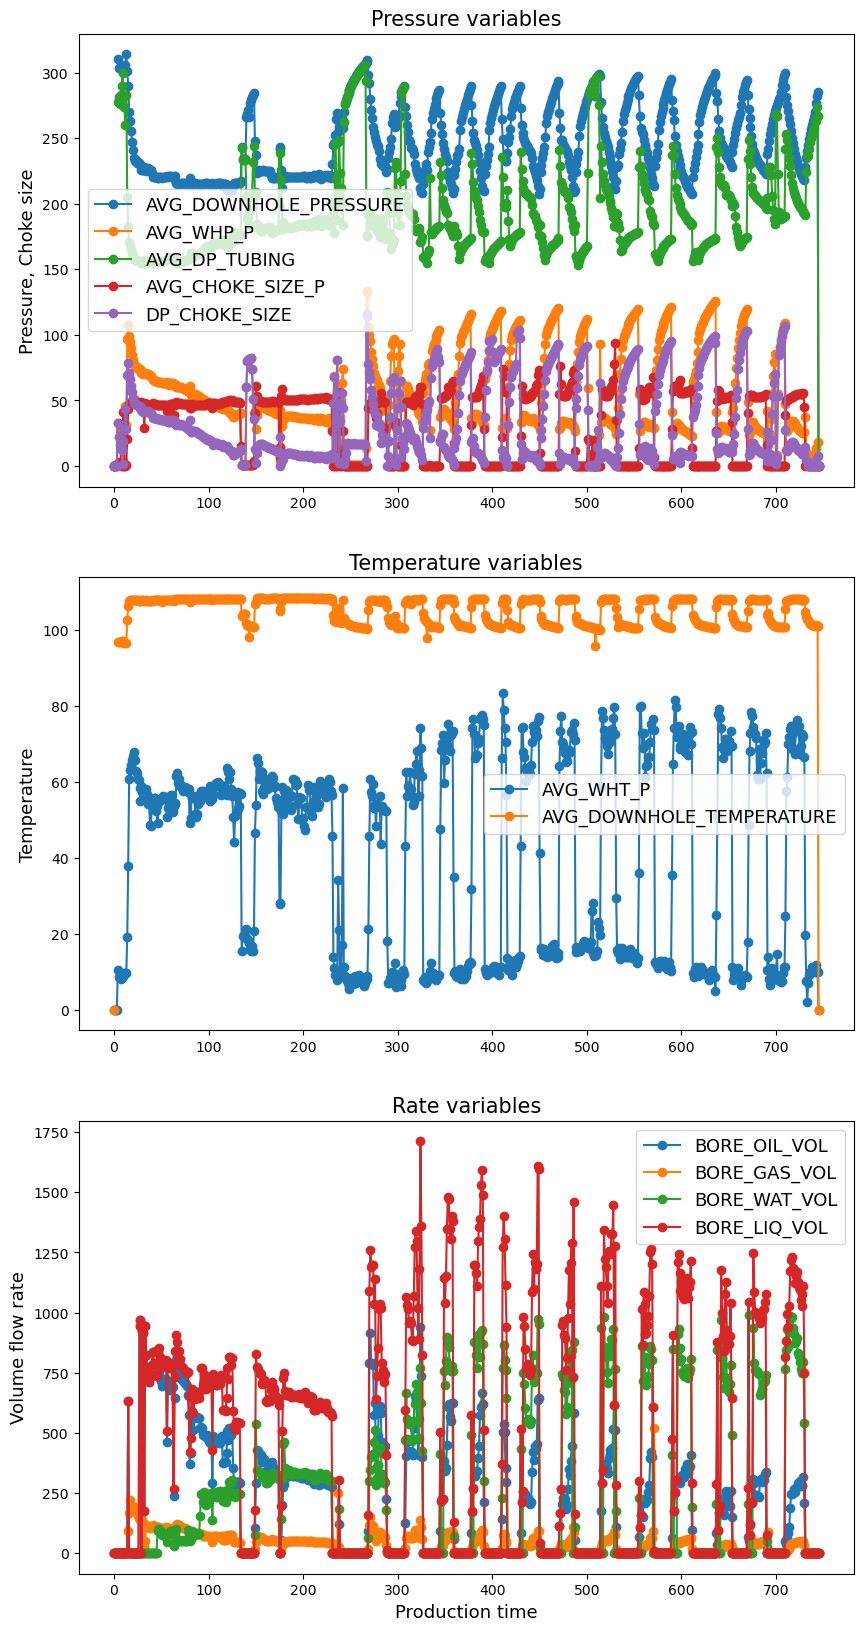
\includegraphics[width=3.5in]{data_example_2.png}}
\caption{Example of well production data available on Volve dataset}
\label{example_well}
\end{figure}

\section{Compared Approaches}\label{sec:compared_approaches}

In this section, the two main approaches compared in this work are presented.

\subsection{System identification approach}

System identification consists on proposing a model (either black box or gray box) that is able
to correctly predict the behaviour of a dynamic system and perform forecasts. The approach tries 
to propose a regression model that can estimate the value of the output variable $y$ in the 
time instant $k$, as shown in equation \ref{eq:sysid_generic}

\begin{equation}\label{eq:sysid_generic}
    y_k = f(\mathbf{X}_{k-1})\,.
\end{equation}

Inspired by the control theory and discrete-time transfer functions, the input vector $\mathbf{X}$
is created by concatenating previous values of the input variable $u$ and the output variable $y$,
as illustrated in equation \ref{eq:sysid_lags}

\begin{equation}\label{eq:sysid_lags}
    \mathbf{X}_k = \
    \begin{bmatrix}
        u_{k} \\ u_{k-1} \\ ... \\ u_{k-n_u} \\ -y_{k} \\ -y_{k-1} \\ ... \\ -y_{k-n_y}
    \end{bmatrix}^T\,.
\end{equation}

When the regression function $f$ is linear, the method is called ARX (\textbf{A}uto\textbf{R}egressive
with E\textbf{X}ogenous variables). When the function is non-linear (usually a polynomial is used)
the method is called NARX (\textbf{N}on-linear ARX). Due to the generic nature of the function $f$,
any regressor (including fully-connected neural networks) can be used to create the model.

Among the advantages of the system identification approach it can be found the simplicity of the model,
its flexibility to different regressors. It is also important to comment that, even thoug equation \ref{eq:sysid_lags}
exemplifies the system identification approach with only a single input and a single output, multiple values of input and
output are also possible by adding more data to the
Some disadvantages of the approach include the need of data
with constant timestepping and, depending on the number of inputs, outputs and lag sizes, the amount of
memory spent in matrix $\mathbf{X}$ in order to store repeated data.

\subsection{Transformer architecture}

The Transformer technology was originally proposed in the article \textbf{Attention is all you need} \cite{attention_is_all},
being originally thought for the task of natural language processing (NLP) and text translation. Ever since, the architecture
saw it's popularity grow exponentially, with usage iven in image processing \cite{transformers_for_images}, a domain historically
dominated by CNNs.

Just like the attention mechanism, transformers make use of the similarity concept to add context to data, allowing better predictions
in sets of inputs. Due to similarities between the NLP and time series in general, the architecture has been proposed as
an alternative to classical deep learning architectures for dealing with time series, like in the works of  Pazouki and Farsani \cite{transformers_ts_forecasting} and 
Zerveas et al. \cite{multivariate_ts_forecasting}.

The proposed architecture for this work is presented in Figure \ref{fig:transformer_architecture}. The architecture consists only of the
Encoder branch of the Transformer model and its input has as features both the inputs and the desired output one timestep before the
desired prediction timestep. It is important to notice that this makes necessary the use of a mask in training time, since for all but
the last timestep in the window (whose prediction is our main objective) the input already contains the desired output.
The possibility of adding some Fully-connected layers after the transformer was also implemented in the model
in order to allow tests with te combination of transformer and MLP architectures.

\begin{figure}[htbp]
    \centerline{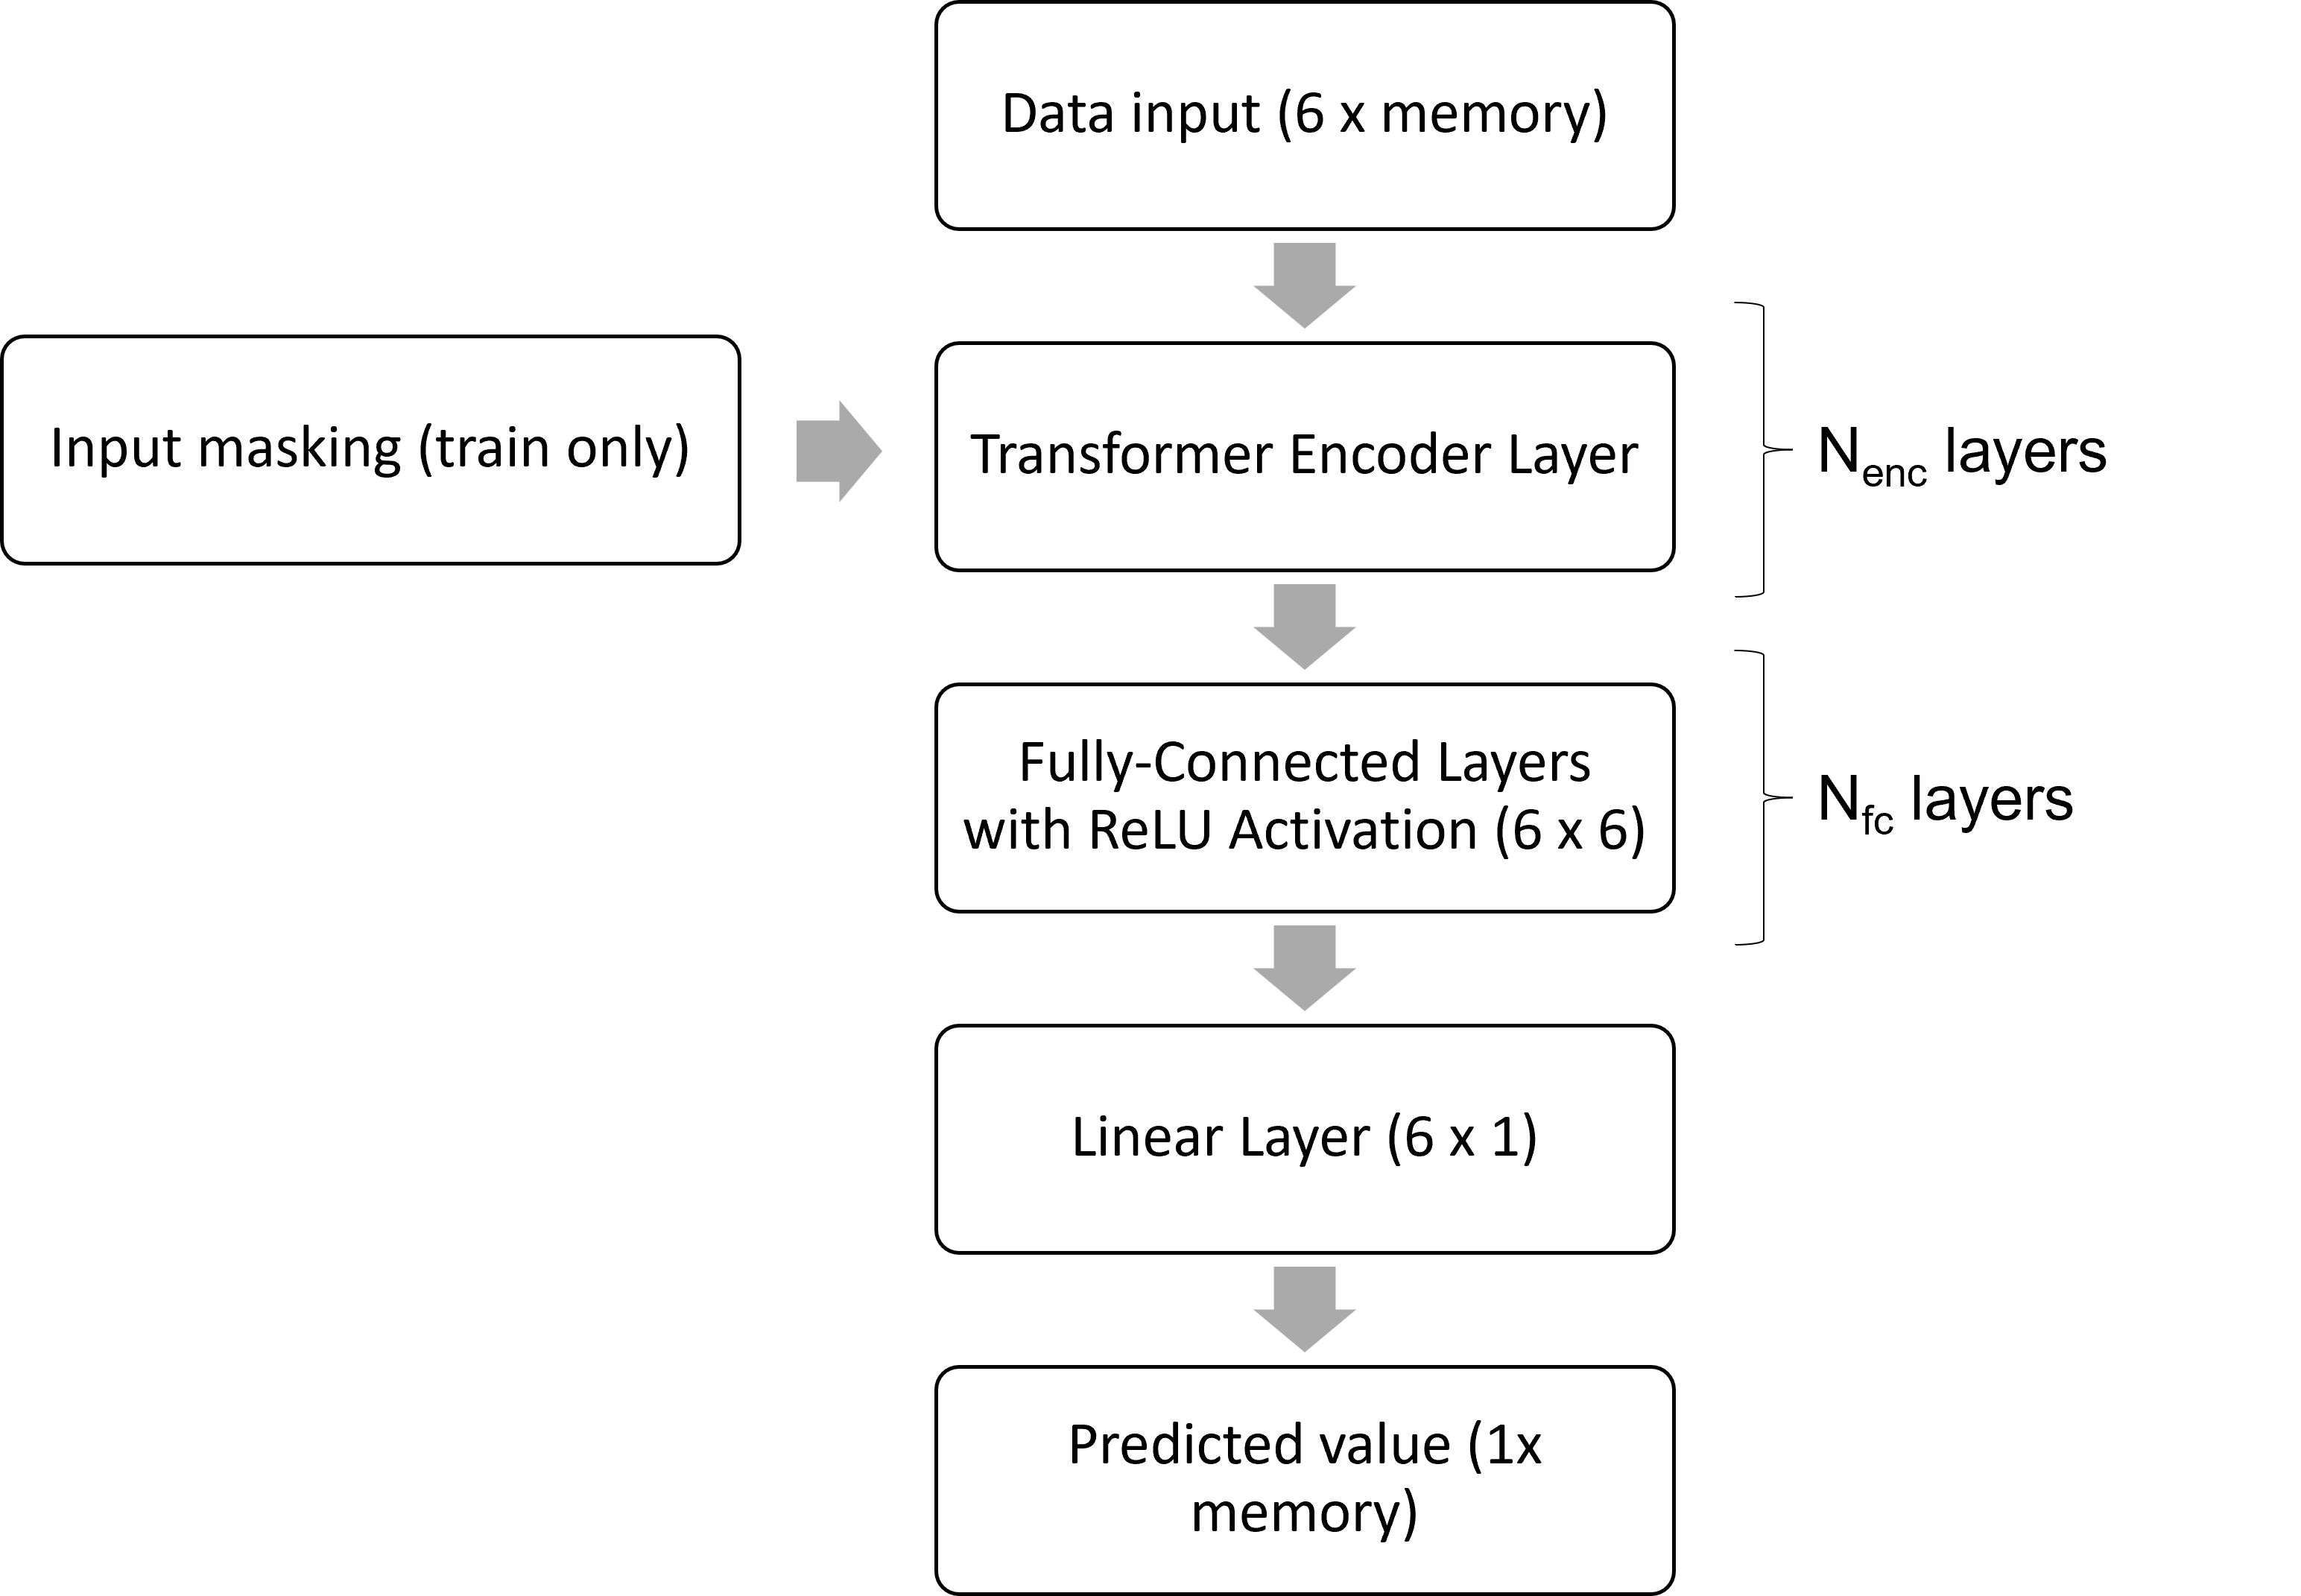
\includegraphics[width=0.48\textwidth]{images/transformer_architecture.png}}
    \caption{Proposed transformer architecture}
    \label{fig:transformer_architecture}
\end{figure}

Due to the relative simplicity of the analyzed problem when compared to the challenges of NLP, some simplifications were made to the
classical transformer architecture. First, no positional encoding was considered in this work, in a way that all the window information
will be equally used to predict the next timestep. Also, since the transformer input was considered to be the normalized features of the timeseries,
and not some sort of encoding of them, the term usually used to correct the effect of the norm in high-dimensionality spaces, $\sqrt{d_k}$,
was also ignored.

When compared to other deep learning architectures used for time series regression and forecasting, such as all variations of
recurrent neural networks, the transformer architecture has the advantage of being fully paralelizable and having essentially
infinite memory (or at least as large as the input window provided). It also shows some advantages when compared with the system
identification approach already presented, since it does not demand a fixed lag size for every prediction and also allows some
some oprimizations in reducing the numper of replicated inputs in the input matrix.

\section{Methodology}\label{sec:section_method}

In this section the general methodology for evaluating and comparing the models will be presented.

\subsection{System identification models}

%The graphical abstract of the system identification model selection pipeline is presented in Figure \ref{fig:graphical_abstract_sysid}.
Since the main scope of this work is to investigate the use of the transformer architecture, no further detail of this approach will be
discussed as it will serve only as a reference for comparison.

%\begin{figure*}[htbp]
%    \centerline{
\includegraphics[width=6.0in]{images/graphical_abstract.png}}
%    \caption{Graphical Abstract and Optimal model selection procedure for the system identification models}
%    \label{fig:graphical_abstract_sysid}
%\end{figure*}

Four regressors will be compared in this approach, all built using the Scikit-learn \cite{sklearn_manual} Python package.
The Table \ref{tab:skl_regressors} shows the estimators considered for comparison.
\begin{table}[htbp]
    \caption{Scikit-learn regressors used for the system identification}
    \begin{center}
    \begin{tabular}{|c|c|}
    \hline
    \textbf{Method}&{\textbf{sklearn regressor}} \\
    \hline
    ARX  & LinearRegression  \\
    \hline
    NARX & PolynomialFeatures + LinearRegression   \\
    \hline
    KNN & KNeighborsRegressor   \\
    \hline
    MLP & MLPRegressor  \\
    \hline
    \end{tabular}
    \label{tab:skl_regressors}
    \end{center}
    \end{table}

\subsection{Transformer models}

Figure \ref{fig:graphical_abstract_transfomers} shows the basic pipeline followed
to train the transformer model. The neural network framework used to implement the 
model was the Pytorch package, with the encoder layer blocks used being the one already 
implemented in the library. A key difference between the transformer pipeline and the
system identification pipeline originally used rests on the normalization step. While 
the system identifications models normalized their data by dividing it by the maximum
value in the time series, for the transformer the 95\% quantile was used, making the absolute values
of the time series to get slightly bigger. This shall be corrected when comparing error
metrics, that wll be discussed in the next section.

\begin{figure*}[htbp]
    \centerline{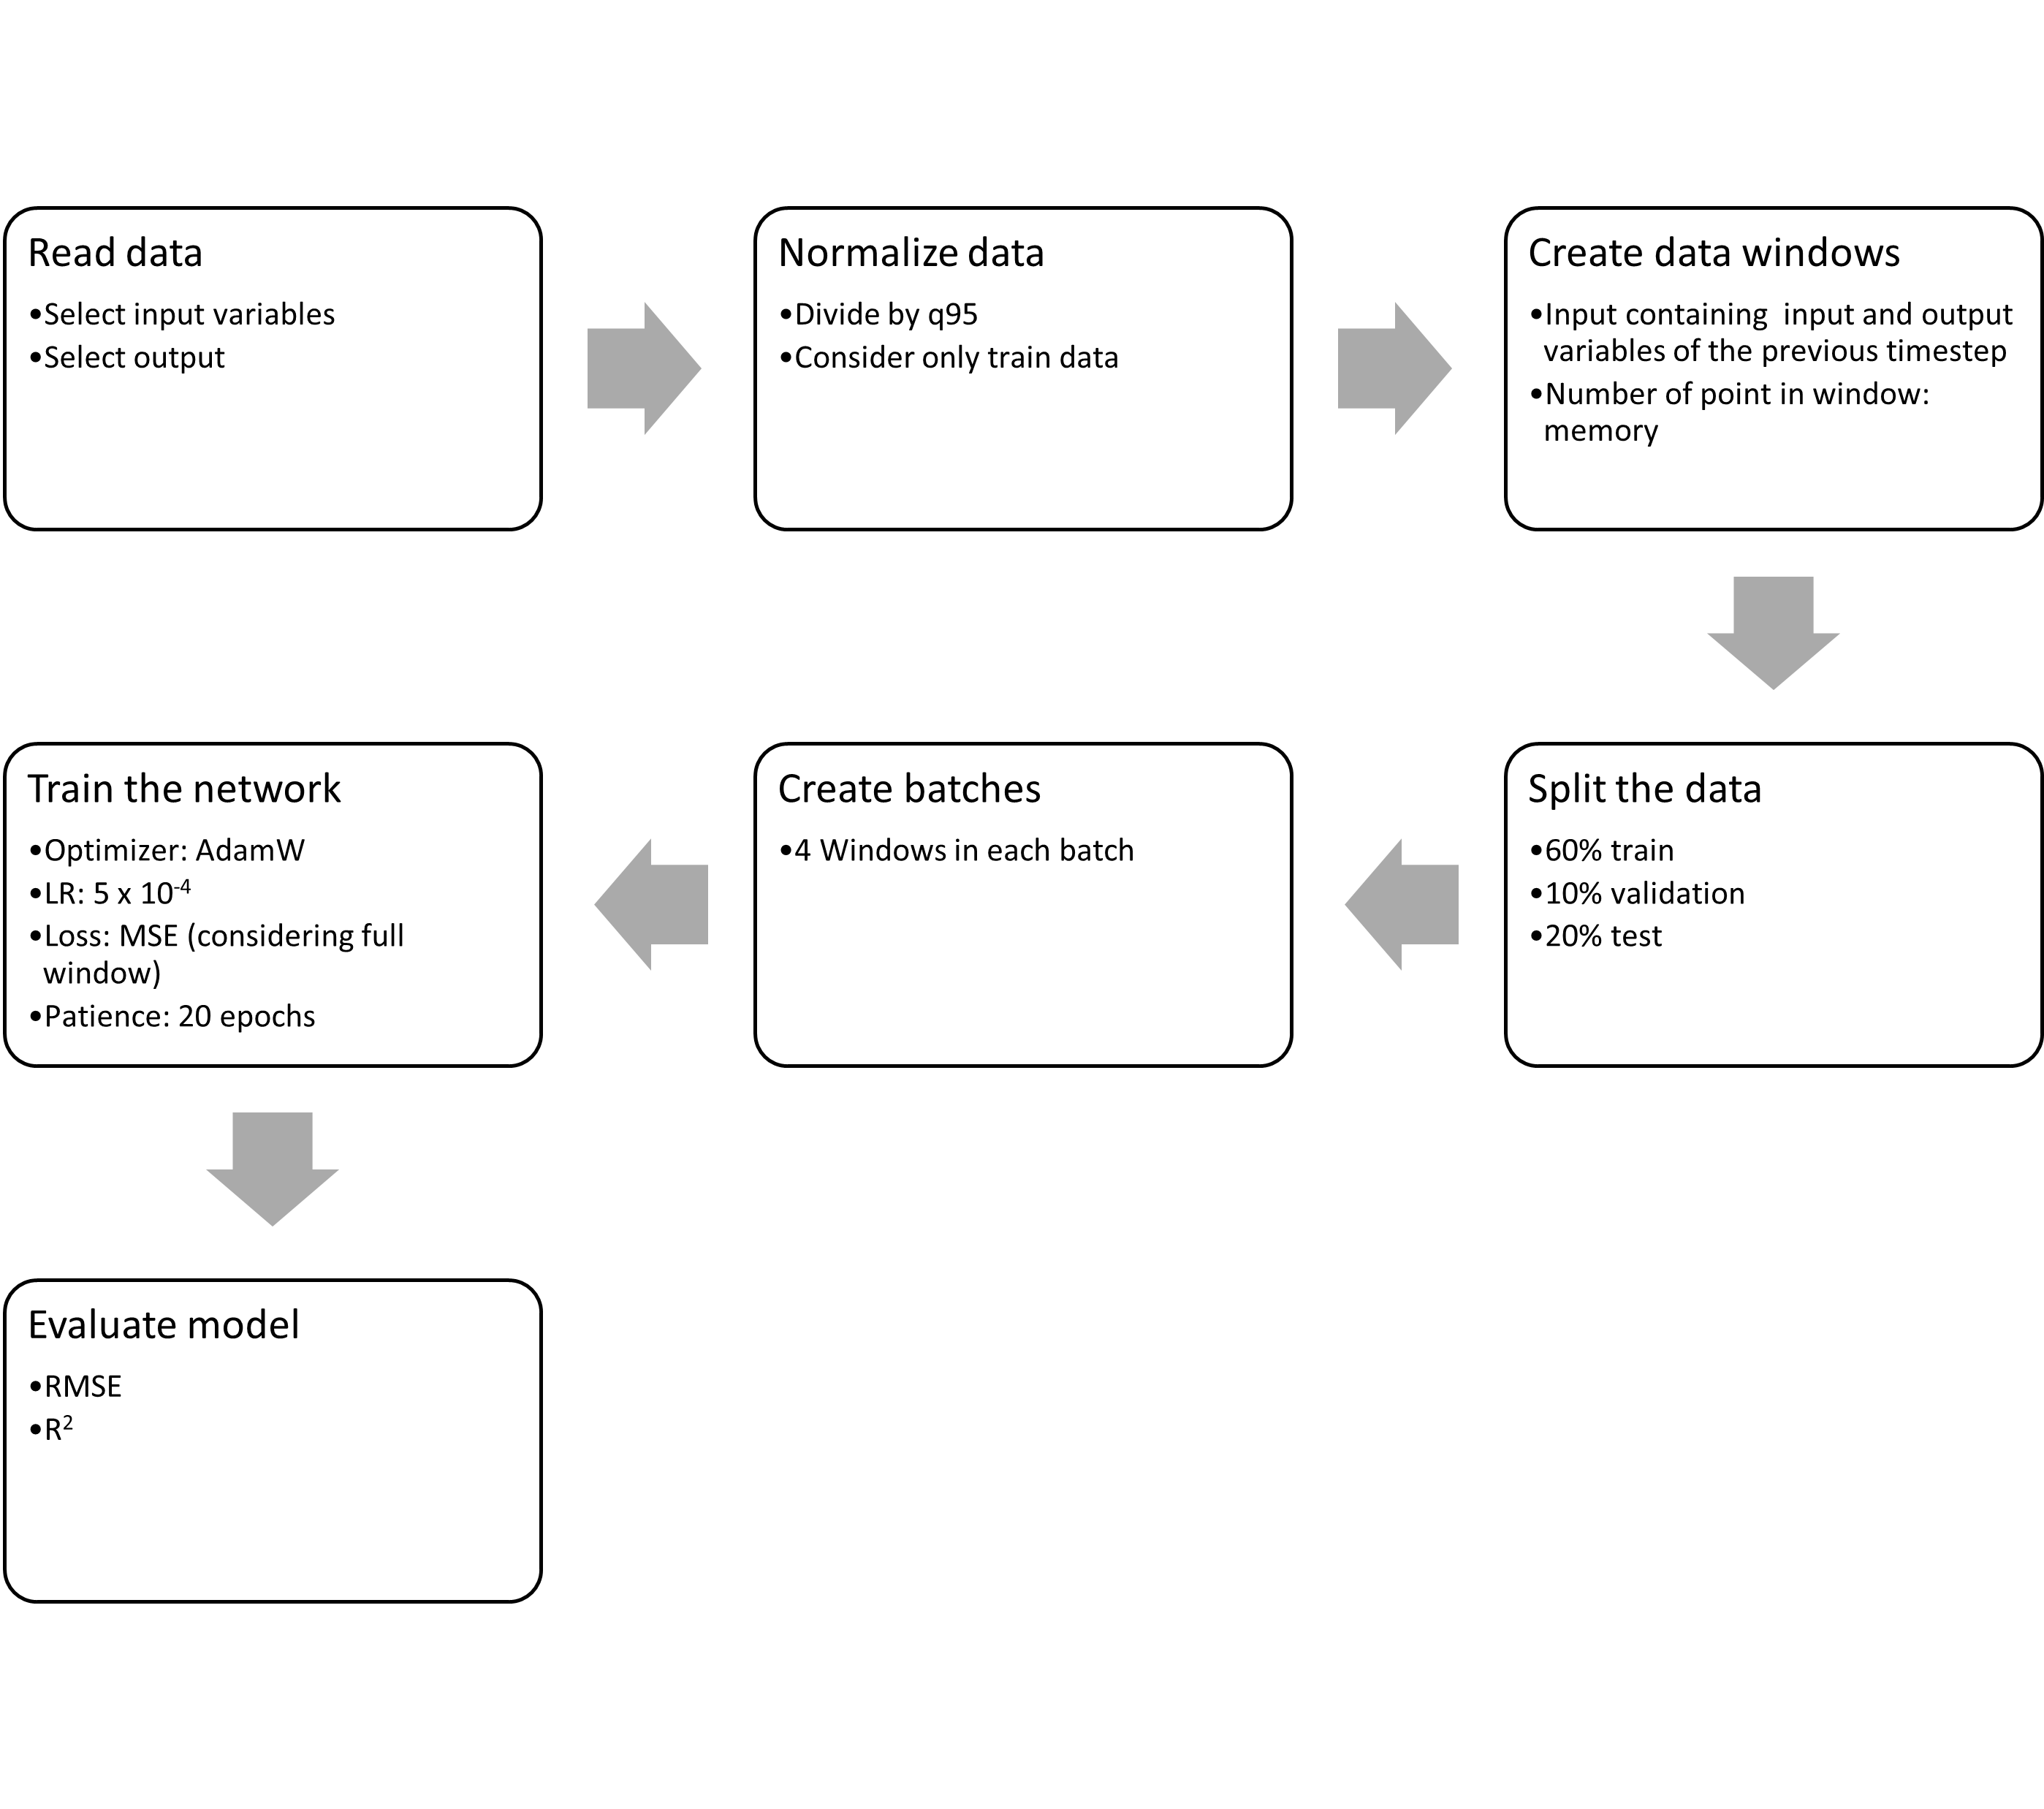
\includegraphics[width=6in]{images/graphical_abstract_transformers.png}}
    \caption{Transformer graphical pipeline}
    \label{fig:graphical_abstract_transfomers}
\end{figure*}

The transformer architecture used in this work allows the variation of the number of
encoder layers and the number of fully-connected layers after the encoder. The training procedure
also allows the variation of the memory used, i.e., the number of vectors passed to the
transformer in order to perform a prediction or train the network. As a base case, a memory window of 16
in a transformer with 1 encoder layer and no fully-connected layer will be considered, but a statistical
analisys with hyperparameter sensitivity will be performed in order to assess the impact of these
choices. It is important to say that, for this work, some parameters of the encoder layer were kept fixed
in all tests, with dropout being fixed in 10\% and feedforward dimension in 12.

In addition to the tests performed considering only data from the reference well, one base case
will also be trained using all the other wells' data in the dataset. In this case, the benchmark
well will only be used as test for the final model. This test aims to evaluate the possibility to apply
transfer learning in this dataset, which can be interesting considering a scenario of
multiple wells in a single reservoir (like it is in Volve). For this test, the base case will
be modified to have 4 encoder alyers, since we have more data to train the model.

\subsection{Error metrics}

The main metric chose to compare the models in this work is the $R^2$ score, showed in equation \ref{eq:r2_eq}

\begin{equation}\label{eq:r2_eq}
    R^2 = 1 - \frac{\sum_{i=1}^N{(y_i - \hat{y}_i})^2}{\sum_{i=1}^N{(y_i - \bar{y})^2}}\,.
\end{equation}

The main advantage of this metric is the fact that it is esencially adimensional and
insensitive to bias and scale errors in the whole timeseries, indicating mainly if the prediction
is able to correctly follow the dynamic of the original data.

Other metrics that will be used to compare the results are the root mean squared error (RMSE), 
defined on equation \ref{eq:rmse_eq} 

%and the residuals auto-correlation defined on equation \ref{autocorr_eq}. The residuals ($\xi$) are defined as de deviation between real values and predicted values and, for a situation where they are purely random, it is expected that their auto-correlation is equal to the Kronecker's delta.

\begin{equation}\label{eq:rmse_eq}
    RMSE = \sqrt{\frac{1}{N}\sum_{i=1}^N{(y_i - \hat{y}_i})^2}\,.
\end{equation}

This metric puts the error in perspective with the scale of data, allowing the comparison
of the error metric with the data values in the dataset, but is necessary to ensure that, in case of comparison,
that both metrics were on the same scale.

One important factor to consider when working with time series forecast is that two types
of predictions are possible. The \textbf{O}ne-\textbf{S}tep \textbf{A}head (OSA) consists in using
real data (form the dataset) from previous timesteps in order to infer ine future timestep. This 
prediction is the one whose error metrics we minimize while performing the training.
The othe is the \textbf{F}ree-run \textbf{S}imulation (FS), which uses only an initial data window
and starts forecasting future timesteps using previous predicitions as starting points. This
prediction tends to be less accurathe than the OSA due to error acumulation, but is far more useful
for engineering purposes since it allows the simulation of long time periods. In this work, the model
ranking will be mostly based in the $R^2$ score for FS simulations.


\section{Results and discussion}\label{sec:section_results}

In this section, the results of the tests performed will be presented, just like the main comparison between the transformer
results and the system identification models.

\subsection{General comparison}

Table \ref{tab:main_results} shows the main comparison results between the models. it is possible to see that the transformer architecture ouperforms
all the evaluated alternatives considering both the $R^2$ and the $RMSE$ for the Free-run Simulation. This is considered the most important case
since it better displays the extrapolation capabilities of the model, while good performance on the One-step Ahead simulation may be an indicative of
overfitting. In fact, it is interesting to notice that considering the metrics for the OSA simulation, the transformer model loses for nearly all the
alternatives in the $RMSE$ comparison ant to the KNN model in the $R^2$ comparison.

\begin{table*}[htbp]
\caption{Metrics results for realized tests}
\begin{center}
\begin{tabular}{|c|c|c|c|c|c|c|c|}
\hline
\textbf{Method,}&\textbf{Model}& \textbf{Regression} &\multicolumn{4}{c|}{\textbf{Total data}}&\textbf{Rank} \\
\cline{4-7} 
\textbf{Inputs} & \textbf{memory}& \textbf{Parameters} &\textbf{\textit{R$^{\mathrm{2}}$ OSA}}& \textbf{\textit{R$^{\mathrm{2}}$ FS}} & \textbf{\textit{RMSE OSA}}& \textbf{\textit{RMSE FS}}& \\
\hline
ARX                                  &  4 &   24 & 0.585 & 0.592 & 0.124 & 0.175&5\\
\hline
NARX                                 &  5 &  496 & 0.655 & 0.662 & 0.119 & 0.159&4\\
\hline
KNN                                  & 20 &    0 & 0.892 & 0.676 & 0.090 & 0.156&3\\
\hline
MLP                                  &  6 & 3281 & 0.723 & 0.688 & 0.105 & 0.153&2\\
\hline
\textbf{Transformer (current work)}  & 16 & 1069 & 0.773 & 0.699 & 0.132$^\mathrm{a}$ & 0.152$^\mathrm{a}$ &1\\
\hline
\multicolumn{7}{l}{$^{\mathrm{a}}$Values corrected considering the different normalizations used in each study} \\
\end{tabular}
\label{tab:main_results}
\end{center}
\end{table*}

Another interesting comparison that can be made is the comparison between the MLP model and the transformer model regarding the number of
regression parameters. Here, it is possible to see that the transformer architecture can better represent the time series dynamics even possessing
less parameters, which serves as an indicative that the architecture is better suited for time series forecasting than the combination of The
system identification approach and a simple fully-connected neural network. Figure \ref{fig:prediction_results} also displays the 
results of the OSA and FS simulations for the transformers model compared with the reference time series, where it is possible to see that
most of the dynamic of the well is captured by the proposed black-box model.

\begin{figure*}[htbp]
    \centerline{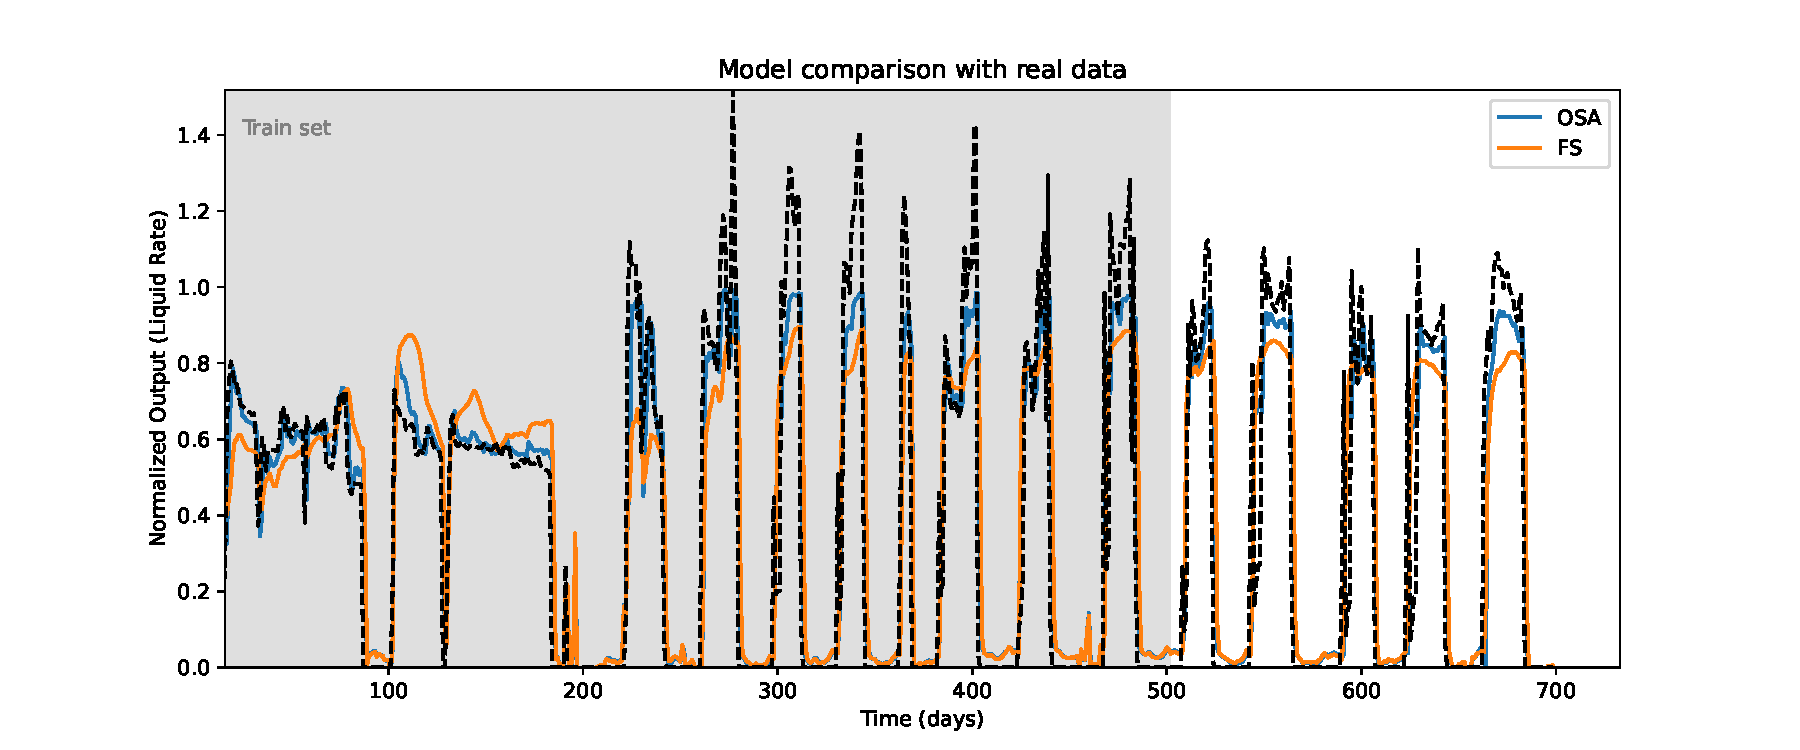
\includegraphics[width=6.0in]{images/prediction_best_model.pdf}}
    \caption{Prediction results for the base transformer case}
    \label{fig:prediction_results}
\end{figure*}

It is also important to notice the importance of the early stopping implemented on the training of the transformer model. Figure \ref{fig:error_convergence} shows
the evolution of the loss function ($MSE$) as the epochs progress. It is already possible to see the start of the overfitting tendency in the graphic for the given 
model training, which could degrade the results if eraly stopping was not used.

\begin{figure}[htbp]
    \centerline{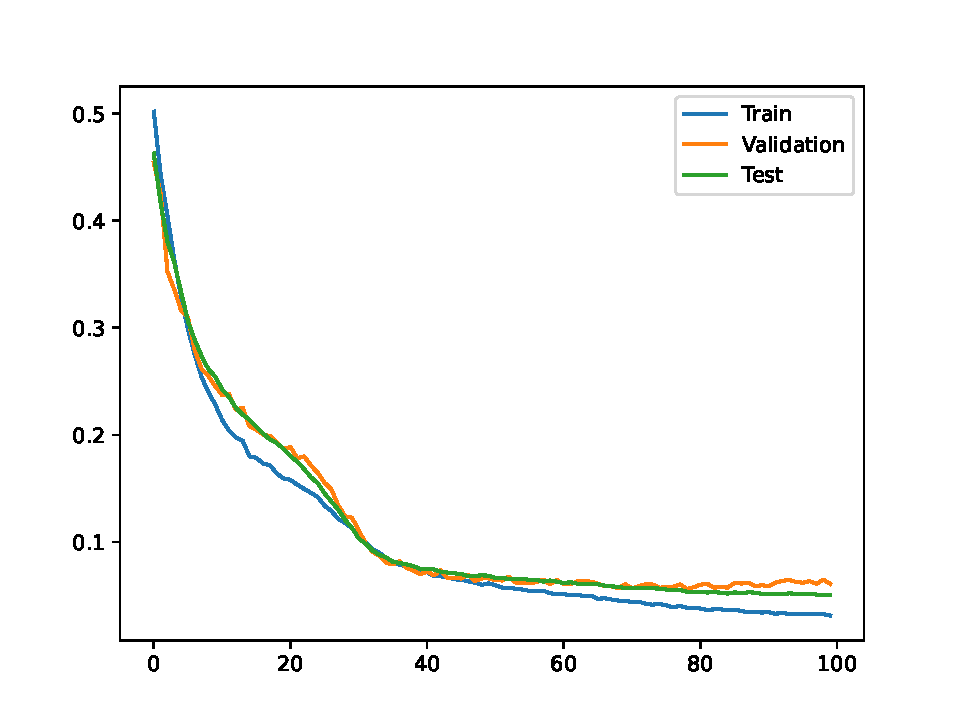
\includegraphics[width=0.49\textwidth]{images/error_convergence.pdf}}
    \caption{Prediction results for the base transformer case}
    \label{fig:error_convergence}
\end{figure}

\subsection{Statistical analysis}

In order to perform some statistical analysis of the transformer model, variations of the proposed transformer were fit multiple times. In each variation, the number of
of encoder layers, the number of fully-connected layers after the transformer and the memory size were altered in order to investigate the impact of these hyperparameters
in the model overall result. Each variatin of the model was fitted 10 times in order to increase the size of the results sample. 

Figure \ref{fig:boxplot_results} displays the boxplot for the considered error metrics in OSA and FS simulations.
Focusing on the FS case, it is possible to notice that both memory and encoder layers have little impact in the mean value
of the metrics with just a slight tendency of improvement for higher values of memory. It is also possible to notice that, 
for cases with more encoder layers, there is a tendency of appearance
of more outliers than in cases with less layers. That is probably due to the small dataset used to train the transformer in this case,
which for cases with large quantities of parameters may not be enough to fit properly the model.

\begin{figure*}[htbp]
    \centering
    \subfloat[$R^2$ boxplot]{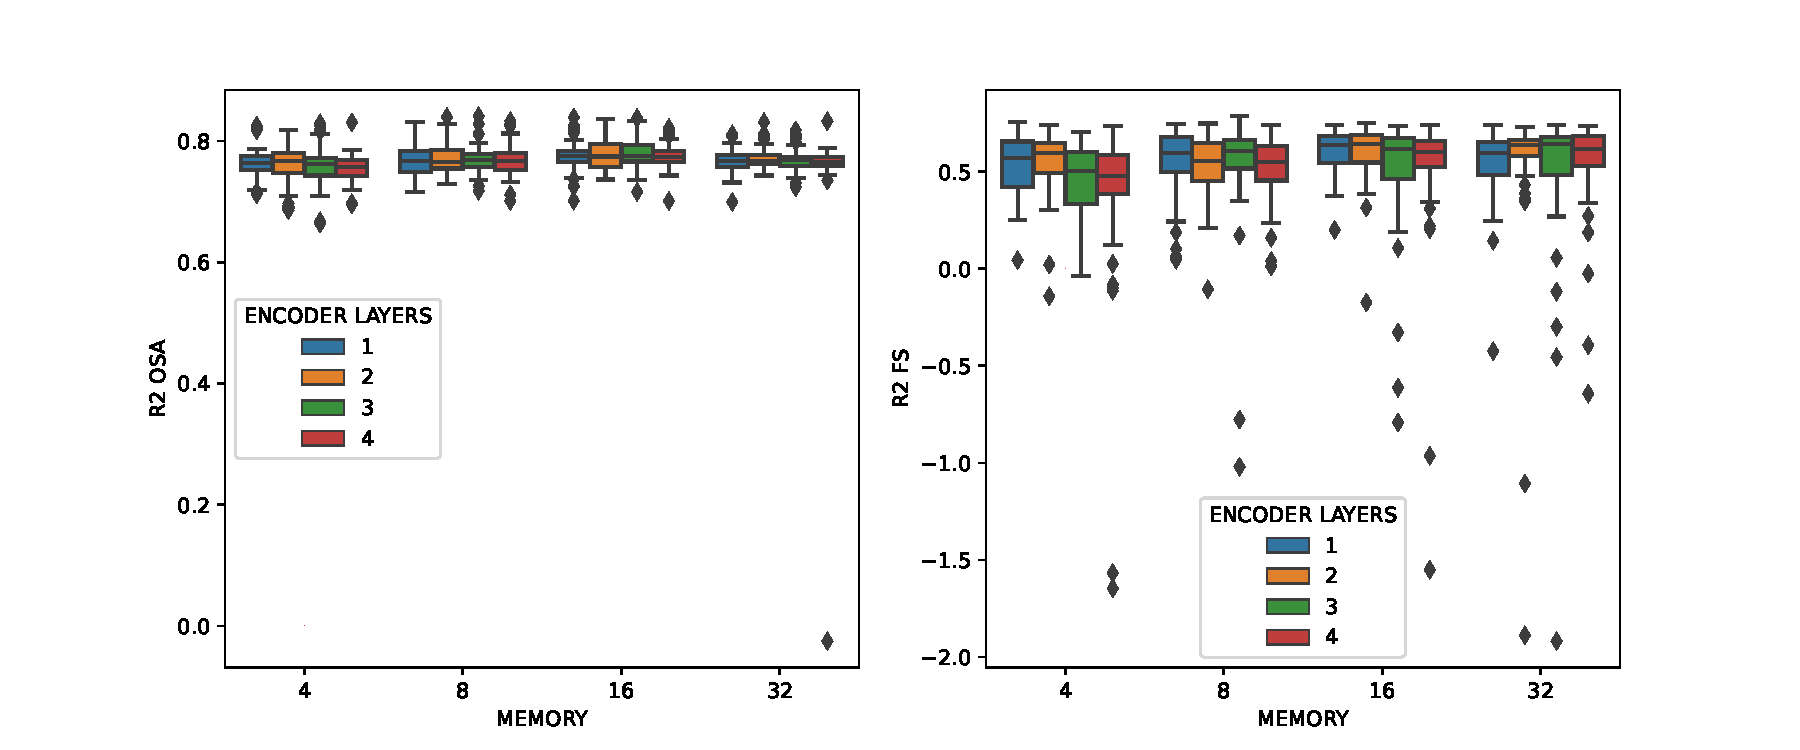
\includegraphics[width=6in]{images/boxplot_MEMORY_R2_ENCODER LAYERS.pdf}\label{fig:box_r2}}
    \hfil
    \subfloat[$RMSE$ boxplot]{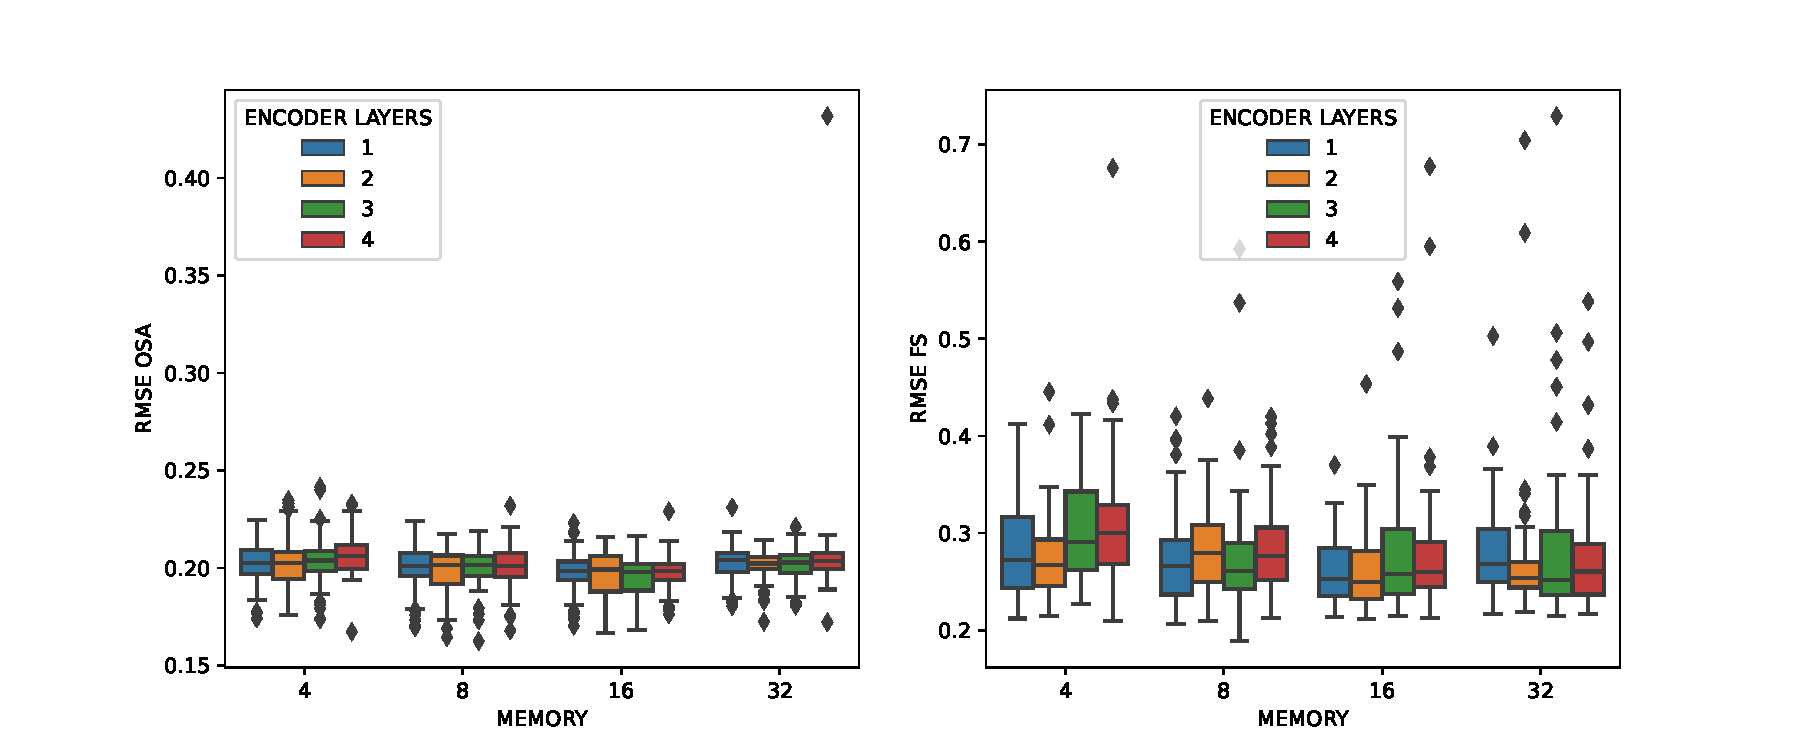
\includegraphics[width=6in]{images/boxplot_MEMORY_RMSE_ENCODER LAYERS.pdf}\label{fig:box_rmse}}
    \hfil
    \caption{Statistical analisys of the impact of memory and number of encoder layers in the results of the model}
    \label{fig:boxplot_results}
\end{figure*}

Figure \ref{fig:statistical_results} represents the mean result from all the runs performed together
with its error bar (here, quantified by the standard deviation of the series) for both all the tested models
and the 10 runs of the reference model only. It is possible to see that for the OSA prediction, as expected,
there is good agerrment and low dispersion in the final responses, while for the FS simulation, the dispersion
is considerably larger. It is also possible to notice that the base case is indeed better, in hte mean, to
predict the results than the average of all the models.

\begin{figure*}[htbp]
    \centering
    \subfloat[All runs]{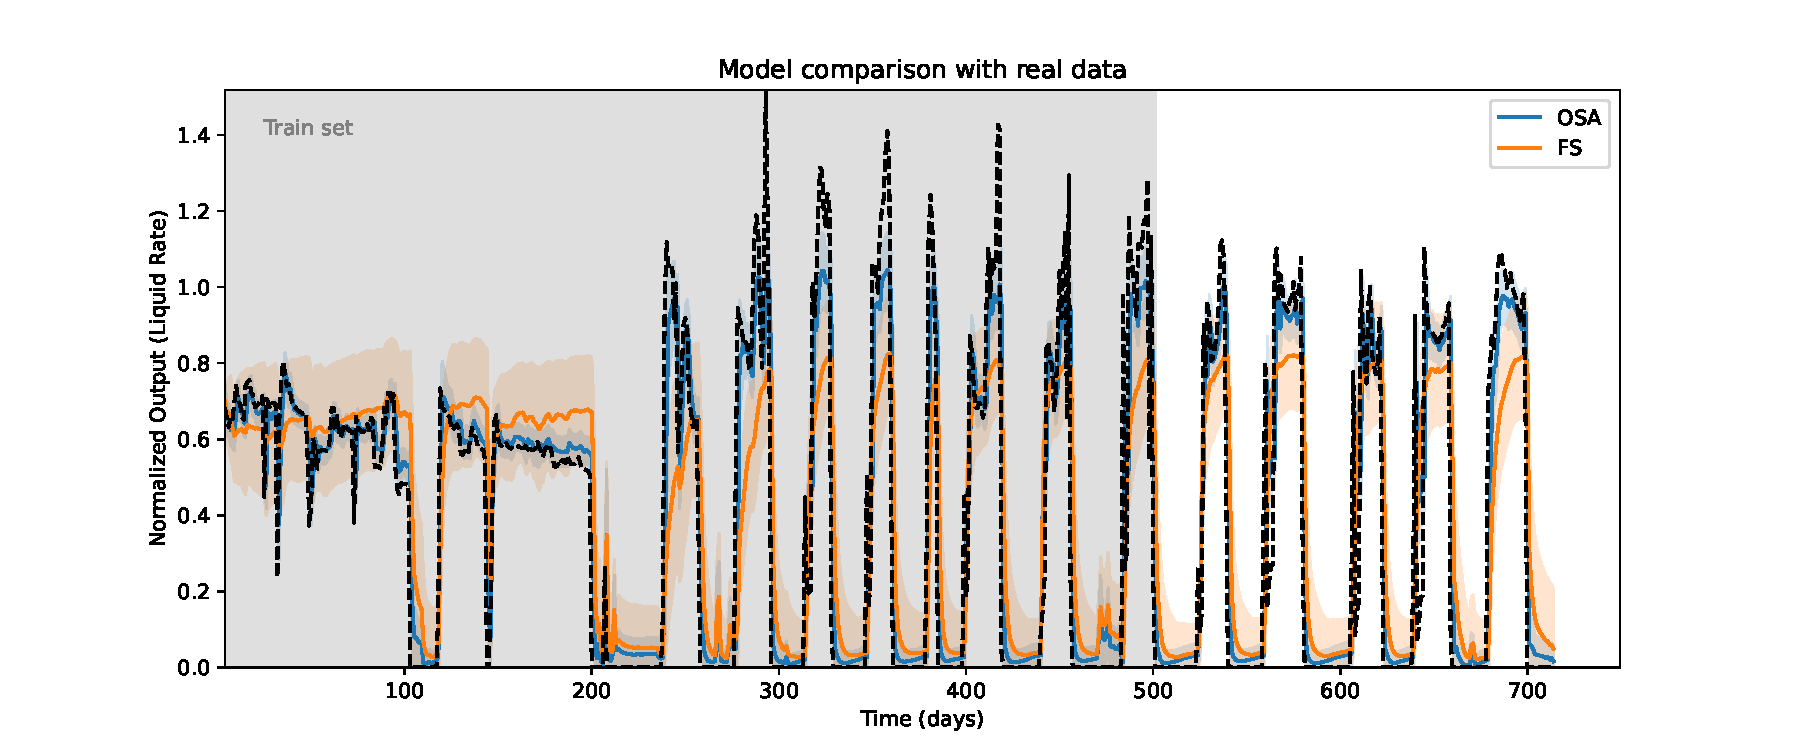
\includegraphics[width=6in]{images/prediction_errorbars.pdf}\label{fig:dispersion_all}}
    \hfil
    \subfloat[Base case runs (memory = 16, encoder layers = 1, linear layers = 0)]{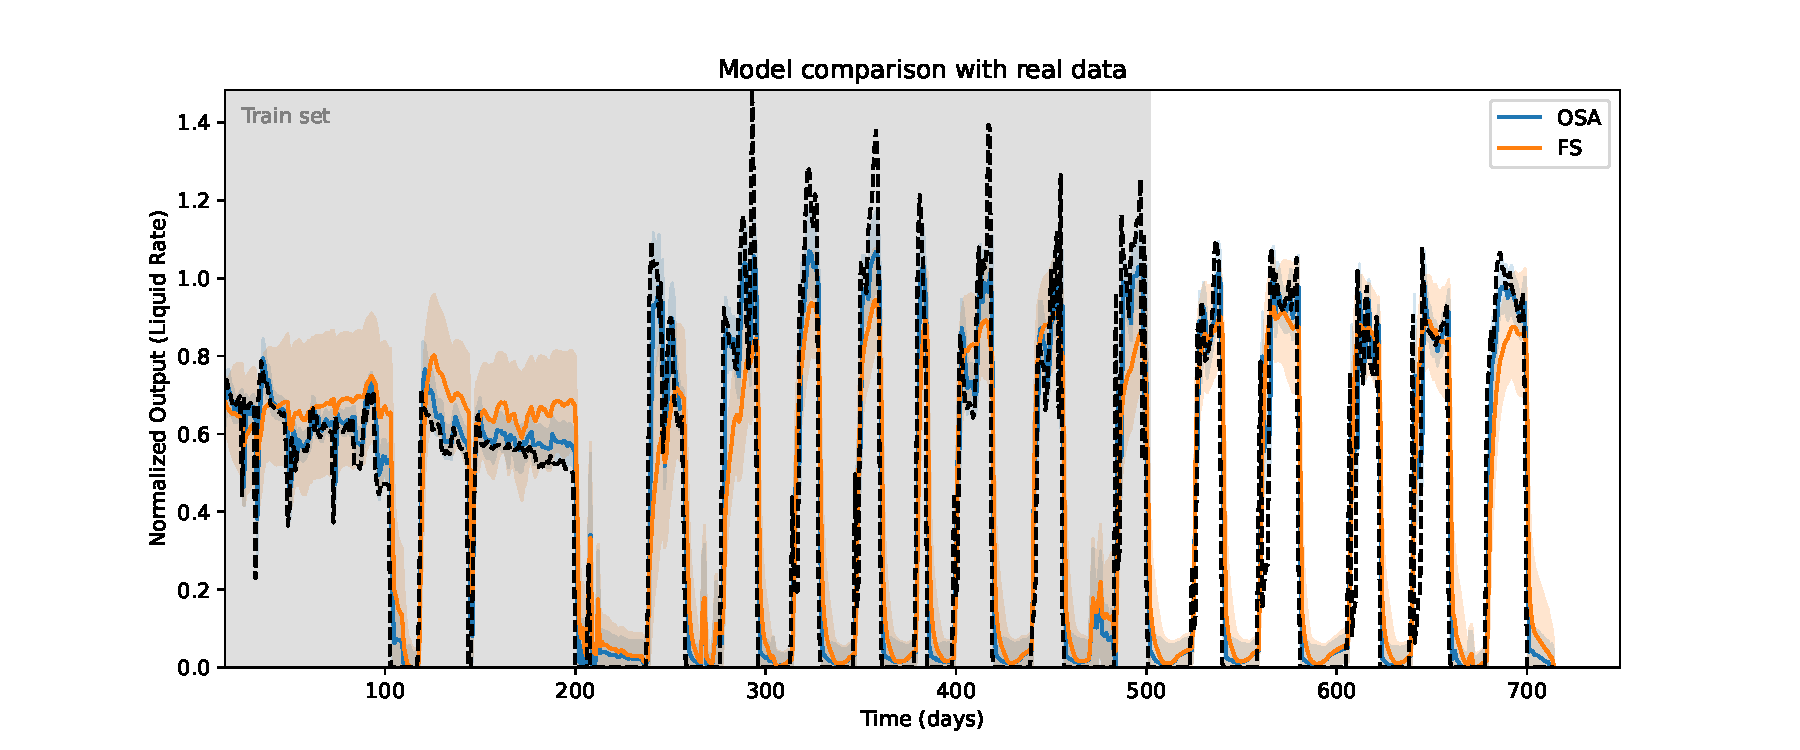
\includegraphics[width=6in]{images/prediction_errorbars_basemodel.pdf}\label{fig:dispersion_base}}
    \hfil
    \caption{Statistical analisys of the impact of memory and number of encoder layers in the results of the model}
    \label{fig:statistical_results}
\end{figure*}

\subsection{Transfer Learning Tests}

In this section, data from the other production wells in the Volve dataset is used to
train our transformer model while the prediction is applied on our benchmark well. 
It is important to emphasize that, in this case, data from the evaluated well is not
seen during the training of the neural network, being used only for test.
Since considering all the wells our dataset gets considerably bigger, for this case a variation
of the base case previously used with 4 encoder layers was adjusted. Figure \ref{fig:tl_prediction_results}
shows the results of the analisys. It is possible to conclude that, while de adopted approach
allowed for good OSA results, predictions done using FS were not as good, being unable to
represent adequately the dynamic of the well.

\begin{figure*}[htbp]
    \centerline{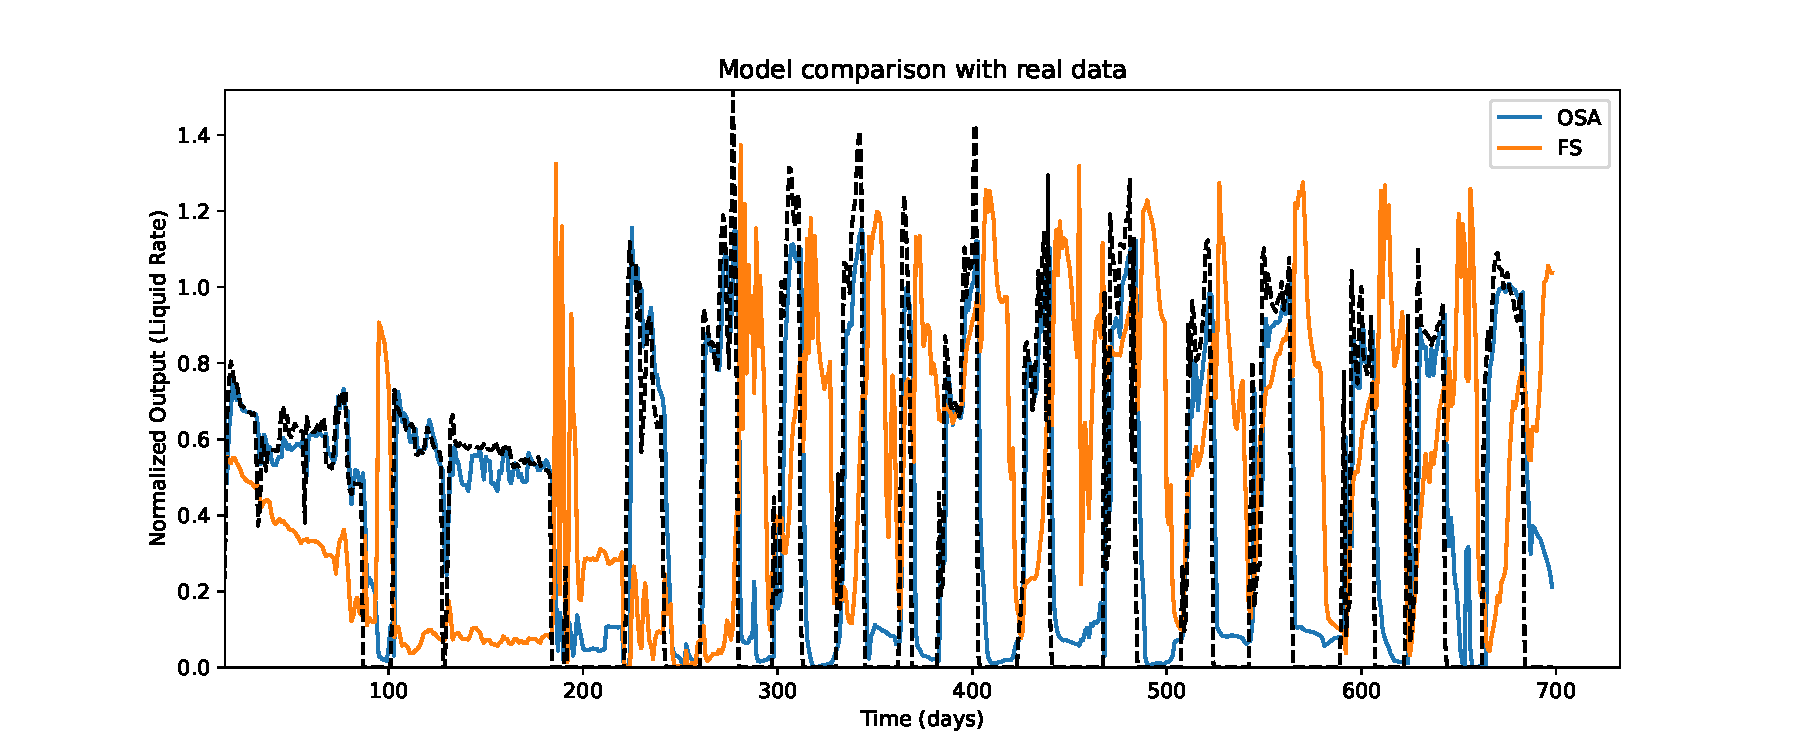
\includegraphics[width=6.0in]{images/multi_best_model.pdf}}
    \caption{Prediction results for the base transformer transfer learning case}
    \label{fig:tl_prediction_results}
\end{figure*}


\section{Conclusion}\label{sec:section_conclusion}

In this work a transformer model was used to create a black-box model for production
forecasting of a well. Statistical analysis of the model was performed together with
with some hyperparameter sensitivities and one simple transfer learning test was performed.

The results obtained indicated that the base model adjusted outperformed the alternatives 
evaluated in metrics for the FS predictions. Comparing with the other neural network model
used as comparison, the transformer architectured showed better performance with less parameters,
indicating that the architecture should be moer adequate to time series forecasting.

The statistical analysis and hyperparameter sensitivity showed that the error metrics were less
sensitive to the memory size and number of encoder layers, but models with more encoder
layers showed more outlier results with poor performance, probably due to the relatively small size of the
time series (around 700 points). Comparing the mean predictions for the base case with the mean
predictions for the whole sensitivity analisys, it is possible to conclude thar, while the
base case seems to, on average, represent better the well dynamics in FS cases, the error bar for both
cases is very similar considering the standard deviation as a metric.

Finally, a version of the base case with more encoder layers was adjusted using the other wells
as training set in order to perform a transfer leraning test. Results show that, while the generated model
can adequately predict the dynamic of the benchmark well in OSA cases, it lacked the extrapolation
capability needed to perform well in FS cases, with further tests and studies to improve this result
being needed.

As a non-exhaustive list of future works following the current paper, it is possible to cite:

\begin{itemize}
    \item Improve the variance of the model, reducing the dispersion
    \item Improve architecture in order to viabilize the transfer learning strategy \
     for Free-run simulations
    \item Work with dimensional data, eliminating the normalization timestep
    \item Include other similar benchmark datasets in the pipeline, such as the SPE Dataset
\end{itemize}



% trigger a \newpage just before the given reference
% number - used to balance the columns on the last page
% adjust value as needed - may need to be readjusted if
% the document is modified later
%\IEEEtriggeratref{8}
% The "triggered" command can be changed if desired:
%\IEEEtriggercmd{\enlargethispage{-5in}}

% references section

% can use a bibliography generated by BibTeX as a .bbl file
% BibTeX documentation can be easily obtained at:
% http://mirror.ctan.org/biblio/bibtex/contrib/doc/
% The IEEEtran BibTeX style support page is at:
% http://www.michaelshell.org/tex/ieeetran/bibtex/
\bibliographystyle{IEEEtran}
% argument is your BibTeX string definitions and bibliography database(s)
% \bibliography{IEEEabrv,../bib/paper}
\bibliography{IEEEabrv,references}
%
% <OR> manually copy in the resultant .bbl file
% set second argument of \begin to the number of references
% (used to reserve space for the reference number labels box)
% \begin{thebibliography}{1}
% \bibitem{IEEEhowto:kopka}
% H.~Kopka and P.~W. Daly, \emph{A Guide to \LaTeX}, 3rd~ed.\hskip 1em plus
%   0.5em minus 0.4em\relax Harlow, England: Addison-Wesley, 1999.
% \end{thebibliography}




% that's all folks
\end{document}
